\documentclass[border=4pt]{standalone}
% Shared typography and colours for the standalone figures.
\usepackage{unicode-math}
\setmainfont{TeX Gyre Termes}
\setmathfont{TeX Gyre Termes Math}
\usepackage{tikz}
\usetikzlibrary{arrows.meta,positioning,calc,decorations.pathreplacing}
\usepackage{pgfplots}
\pgfplotsset{compat=1.18}

% One colour per element or subsystem. Record the mapping in
% the working repository conventions and use it identically in every figure.
\definecolor{elemA}{HTML}{1F5FA8}
\definecolor{elemB}{HTML}{B8461B}
\definecolor{elemC}{HTML}{2E7D32}
\definecolor{elemD}{HTML}{6A4C93}
\definecolor{frameline}{HTML}{555555}

\begin{document}
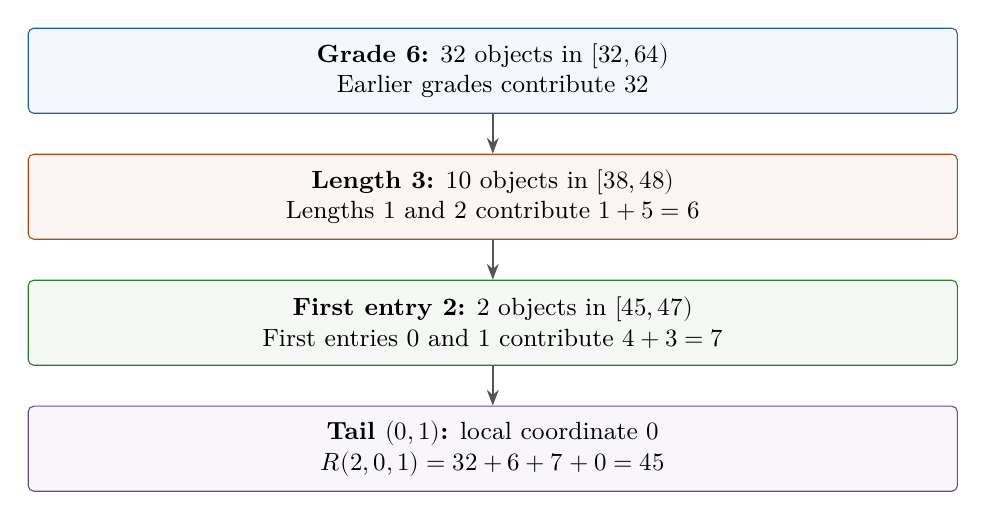
\begin{tikzpicture}[
 font=\small,
 box/.style={draw,rounded corners=2pt,minimum width=11.8cm,minimum height=1.08cm,align=center},
 arr/.style={-{Stealth[length=2mm]},thick,frameline}]
\node[box,draw=elemA,fill=elemA!5] (a) at (0,0)
  {\textbf{Grade 6:} 32 objects in $[32,64)$\\Earlier grades contribute $32$};
\node[box,draw=elemB,fill=elemB!5] (b) at (0,-1.6)
  {\textbf{Length 3:} 10 objects in $[38,48)$\\Lengths 1 and 2 contribute $1+5=6$};
\node[box,draw=elemC,fill=elemC!5] (c) at (0,-3.2)
  {\textbf{First entry 2:} 2 objects in $[45,47)$\\First entries 0 and 1 contribute $4+3=7$};
\node[box,draw=elemD,fill=elemD!5] (d) at (0,-4.8)
  {\textbf{Tail $(0,1)$:} local coordinate $0$\\$R(2,0,1)=32+6+7+0=45$};
\draw[arr] (a)--(b);\draw[arr] (b)--(c);\draw[arr] (c)--(d);
\end{tikzpicture}
\end{document}
